% !TEX root = ../main.tex

\clearpage
% Source PDF page 2.
\section*{《捧腹大笑思想与奶龙学概论》第一版前言}
\pdfbookmark[1]{《捧腹大笑思想与奶龙学概论》第一版前言}{preface}

\begin{center}
\textbf{编者：Tono\_Hanna、Chishoo、Tachibana\_Sherry}
\end{center}

\begin{center}
\textbf{特别感谢 BUAA 奶龙同好会喵！}
\end{center}

我一直想为奶蛙作传。

在去年的时候，我在 QQ 水群看到了一张图片：

% !TEX root = ../../main.tex
\begin{figure}[H]
  \centering
  \phantomsection
  \addcontentsline{lof}{figure}{\protect\numberline{}前言插图: 奶龙学概论书影}
  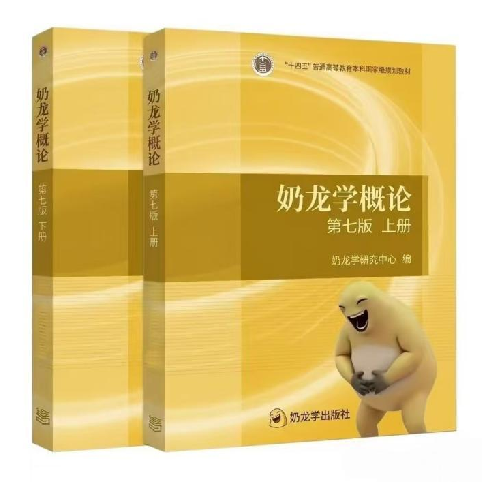
\includegraphics[width=165bp,height=0.76\textheight,keepaspectratio]{figures/preface/preface.pdf}
\end{figure}


自己将自己的所见所闻总结为一本书——更准确地说，是一本课本——让别人看这些东西，体会自己的感受，这件事对我来说一直都是一件趣事。只不过在高考结束前，我一直没有时间和契机去做这件事情。奶龙和奶蛙前所未有的爆火，和 BUAA 奶龙同好会积极的氛围，让我在大学终于找到了这样一个机会。

奶蛙作为纯粹快乐情绪的代言人，在中国的大学生们之间大受欢迎到了这种地步，细想其实是一件有些可悲的事情。但不管怎样，大家在前所未有的变局时代能够找到这样一个快乐的源泉，这是好事啊。

不管怎么样，无论你是资深的奶蛙大手子，还是被刷屏但是没有深入了解的小白（这个可能应该不大吧），你将会在这本“书”中学习系统的奶龙和奶蛙知识，了解奶龙和奶蛙的来龙去脉，并且对捧腹大笑这一看似无厘头的行为有更加深入的理解。

在本书第一章，你将会了解当下奶龙和奶蛙的影响力；在第二章到第四章，我们将会讨论奶龙、奶蛙、捧腹大笑的发展史；在第五章，我们会系统分析捧腹大笑的心理作用；在第六章到第七章，你将会了解奶蛙除了捧腹大笑外的其他表现形式；在第八章，你将会了解奶蛙商品在现实中的情况；在第九章，你将会了解一些高校的奶蛙活动情况。

希望在阅读完本书后，你将会对奶蛙有更加深入的认识，并且让自己的生活更加快乐。

哪怕只是一瞬间，也请忘掉令你烦恼的一切，发自内心地捧腹大笑吧。

《捧腹大笑思想与奶龙学概论》最新版网址：

\url{https://github.com/Chishoo/The-Study-of-Hilarious-Thoughts-and-Milkfrog}

\begin{flushright}
By Chishoo, 2026/9/29
\end{flushright}

